\item \textbf{Try modeling the residuals as an AR process. Use the tools at your disposal to decide on an appropriate order and analyse the results. What is the impact of selecting different orders on the remaining residuals?}





%so these are my starting points
%must be stationary
%these two plot do not tell us much
\textit{For this part, we need to select the order of the \gls{AR} term (p). Therefore, \gls{PACF} and \gls{ACF} were plotted at first step (see figures \ref{fig:Ass1_D1_PACF_ACF_X} and \ref{fig:Ass1_D2_PACF_ACF_X}).}  

\begin{figure}[H]
    \centering
    \begin{minipage}[b]{1\textwidth}
        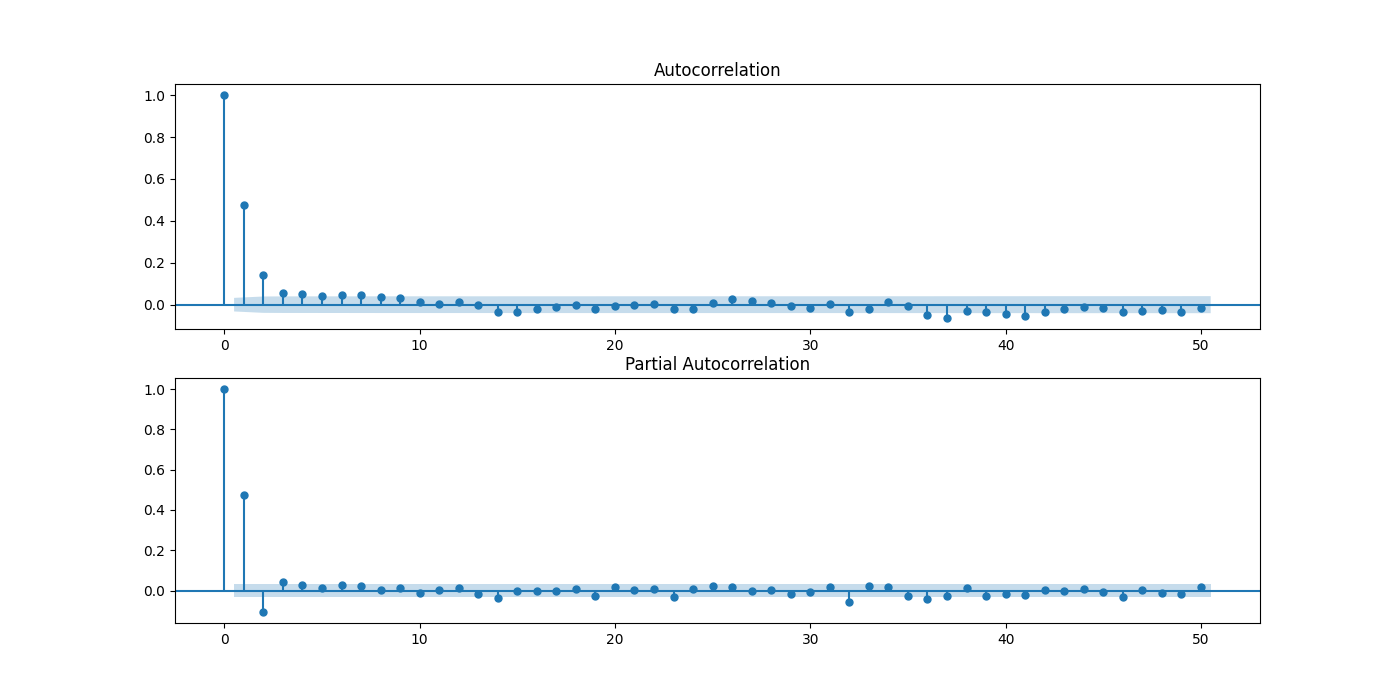
\includegraphics[width=\textwidth]{figures/Ass1/Ass1_D1_PACF_ACF_X.png}
    \end{minipage}
    \caption{A plot of the \gls{PACF} and \gls{ACF} of the residual part of the first dataset (residual of the STL method).}
    \label{fig:Ass1_D1_PACF_ACF_X}
\end{figure}

\begin{figure}[H]
    \centering
    \begin{minipage}[b]{1\textwidth}
        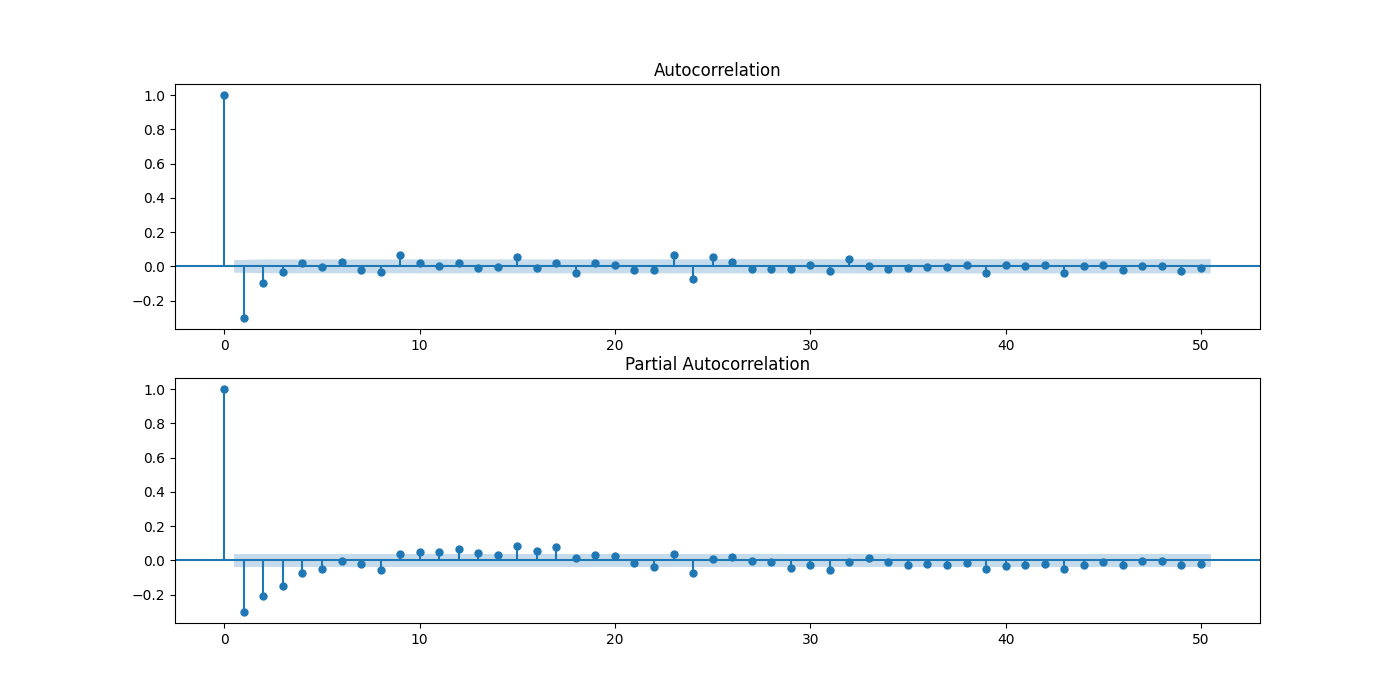
\includegraphics[width=\textwidth]{figures/Ass1/Ass1_D2_PACF_ACF_X.png}
    \end{minipage}
    \caption{A plot of the \gls{PACF} and \gls{ACF} of the residual part of the second dataset (residual of the STL method).}
    \label{fig:Ass1_D2_PACF_ACF_X}
\end{figure}


\textit{Sinse \gls{ACF} decaying in both figures, it can be concluded that the process is an Auto Regressive process. Also, based on \gls{PACF} in the first plot (figure \ref{fig:Ass1_D1_PACF_ACF_X}), the parameter of the \gls{AR} model should be start with lags 1 and 2 due to these two lags have a significant value. Likewise, for the second dataset, we should start with lags 1 to lags 4 (see figure \ref{fig:Ass1_D2_PACF_ACF_X}).}

\begin{figure}[H]
    \centering
    \begin{minipage}[b]{1\textwidth}
        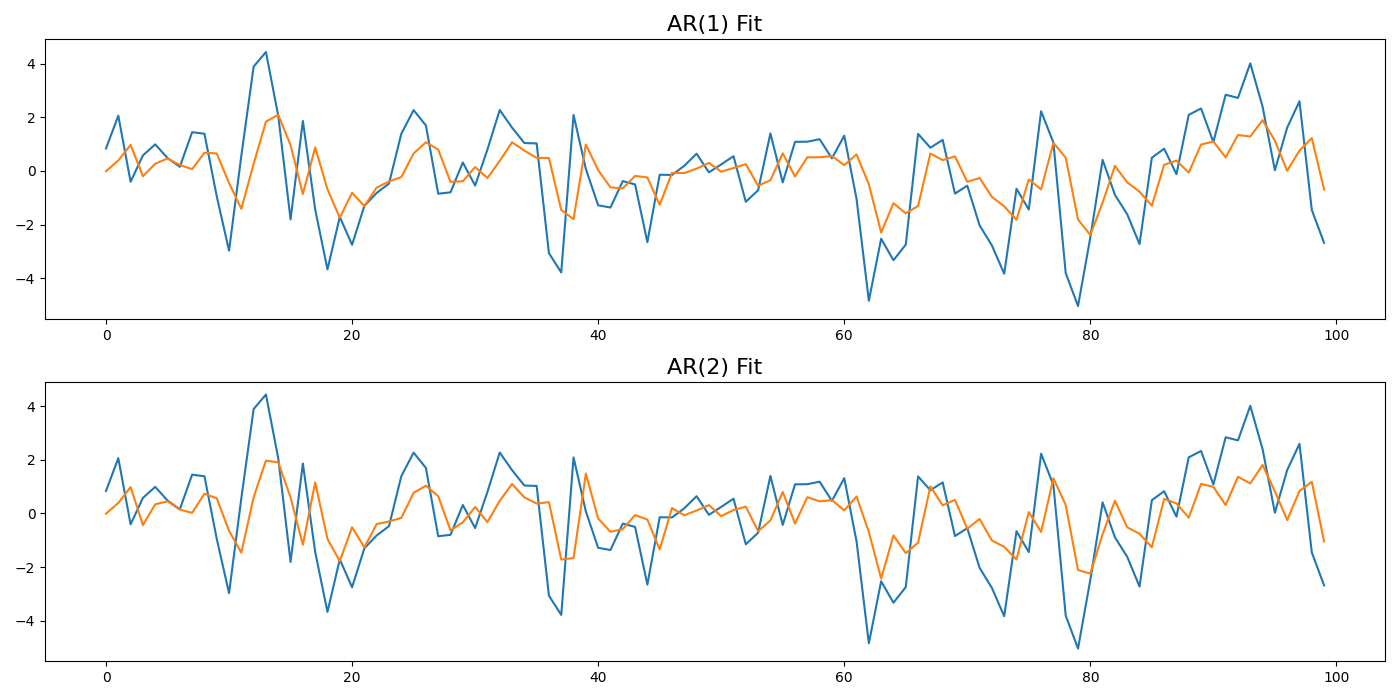
\includegraphics[width=\textwidth]{figures/Ass1/Ass1_D1_ARs models.png}
    \end{minipage}
    \caption{The residual signal (blue) and the prediction of \gls{AR} (orange) for the first dataset.}
    \label{fig:Ass1_D1_ARs_models}
\end{figure}

\begin{figure}[H]
    \centering
    \begin{minipage}[b]{1\textwidth}
        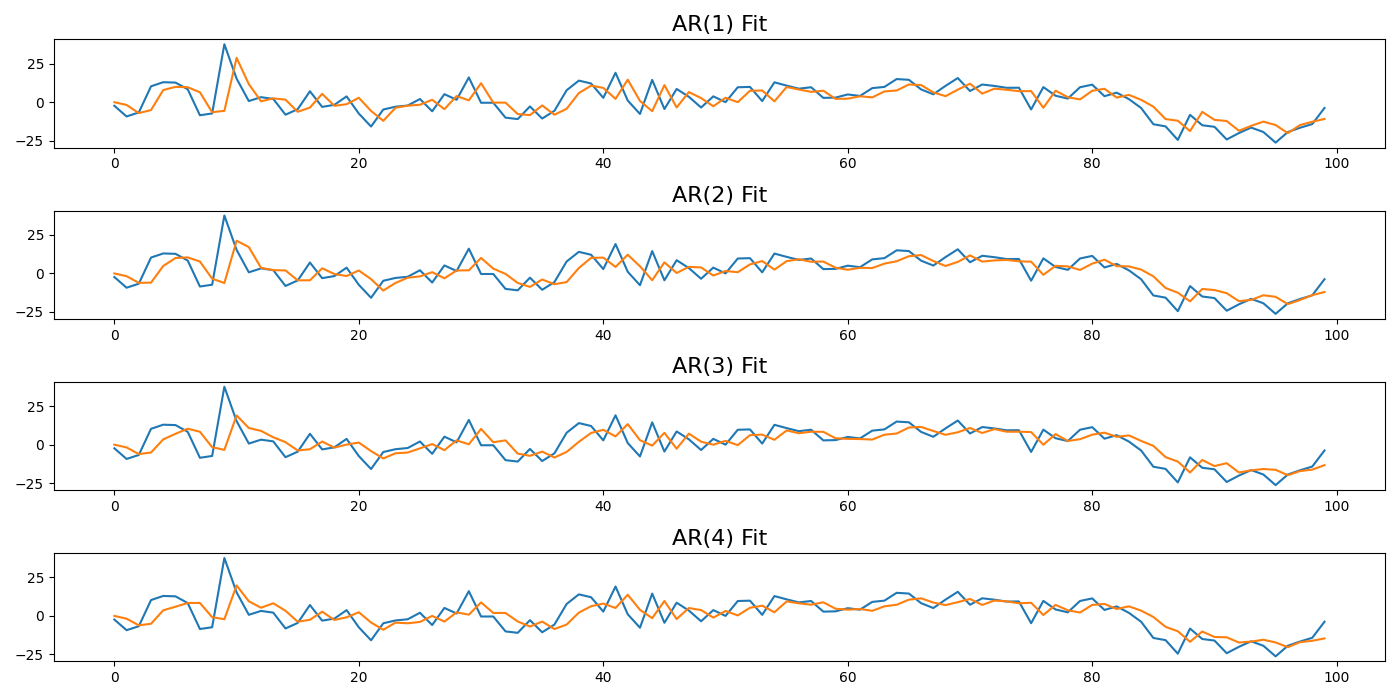
\includegraphics[width=\textwidth]{figures/Ass1/Ass1_D2_ARs models.png}
    \end{minipage}
    \caption{The residual signal (blue) and the prediction of \gls{AR} (orange) for the second dataset.}
    \label{fig:Ass1_D2_ARs_models}
\end{figure}


\textit{Figure \ref{fig:Ass1_D1_ARs_models} and \ref{fig:Ass1_D2_ARs_models} indicate the output of our models on the datasets. In addition, tables \ref{tab:Ass1_D1_AR} and \ref{tab:Ass1_D2_AR} show others parameters of these models. }

\begin{table}[H]
\centering
\caption{Comparing the \gls{AR} models in the first dataset.}
\label{tab:Ass1_D1_AR}
\begin{tabular}{lll}
\toprule
{} &  AR(1) &  AR(2) \\
\midrule
AR order  &      1 &      2 \\
AIC       &  1.288 &  1.277 \\
BIC       &  1.293 &  1.284 \\
RMS error &  1.149 &  1.156 \\
\bottomrule
\end{tabular}

\end{table}

\begin{table}[H]
\centering
\caption{Comparing the \gls{AR} models in the second dataset.}
\label{tab:Ass1_D2_AR}
\begin{tabular}{lllll}
\toprule
{} &      AR(1) &      AR(2) &      AR(3) &      AR(4) \\
\midrule
lag(s)      &          1 &          2 &          3 &          4 \\
AIC         &  22359.771 &  22236.837 &  22136.843 &  22097.596 \\
BIC         &  22377.589 &  22260.594 &  22166.538 &  22133.231 \\
RMS error   &      7.777 &      8.629 &     10.069 &     11.047 \\
Correlation &      0.522 &      0.457 &      0.401 &      0.335 \\
MPE         &     -0.618 &      0.046 &      0.739 &      1.149 \\
MAE         &      5.994 &      6.706 &      7.953 &      9.017 \\
\bottomrule
\end{tabular}

\end{table}







\textit{\Gls{AIC} and \gls{BIC} that show simplicity and goodness of a \gls{AR} model. The model that has a lower \gls{AIC} and \gls{BIC} is generally better than others for example, AR() .}